\documentclass[11pt]{article}
\usepackage{fullpage}
\usepackage[utf8]{inputenc}
\usepackage{amsmath}
\usepackage{amsthm}
\usepackage{amsfonts}
\usepackage{amssymb}
\usepackage{graphicx}
\usepackage{hyperref}
\usepackage{algorithm}
\usepackage{algpseudocode}
\usepackage{listings}
\usepackage{color}
\usepackage{float}
\usepackage{tikz}
\usepackage{tikz-qtree}
\usepackage{mdframed}
\usepackage{pgfplots}
\makeatletter
\newenvironment{breakablealgorithm}
  {% \begin{breakablealgorithm}
   \begin{center}
     \refstepcounter{algorithm}% New algorithm
     \hrule height.8pt depth0pt \kern2pt% \@fs@pre for \@fs@ruled
     \renewcommand{\caption}[2][\relax]{% Make a new \caption
       {\raggedright\textbf{\ALG@name~\thealgorithm} ##2\par}%
       \ifx\relax##1\relax % #1 is \relax
         \addcontentsline{loa}{algorithm}{\protect\numberline{\thealgorithm}##2}%
       \else % #1 is not \relax
         \addcontentsline{loa}{algorithm}{\protect\numberline{\thealgorithm}##1}%
       \fi
       \kern2pt\hrule\kern2pt
     }
  }{% \end{breakablealgorithm}
     \kern2pt\hrule\relax%
   \end{center}
  }
\makeatother
\newtheoremstyle{definitionstyle}
  {3pt} % Space above
  {3pt} % Space below
  {\normalfont} % Body font
  {} % Indent amount
  {\bfseries} % Theorem head font
  {} % Punctuation after theorem head
  { } % Space after theorem head
  {} % Theorem head spec (can be left empty, meaning `normal`)

\theoremstyle{definitionstyle}
\newtheorem{defn}{Definition}
\newtheorem{thm}{Theorem}
% \newtheorem{proof}{Proof}
\usepackage{framed}
\newenvironment{framedminipage}
    {\begin{framed}\begin{minipage}{0.9\textwidth}}
    {\end{minipage}\end{framed}}
\begin{document}
\title{A Dive to MCTS}
\author{liuhanzuo}
\date{\today}
\maketitle
\begin{abstract}
In this survey, we delve into the intricacies of Monte Carlo Tree Search (MCTS), a powerful algorithmic framework used for decision-making in various domains. We begin by exploring the foundational concepts of Markov Decision Processes (MDP) and Monte Carlo methods, which underpin MCTS. The survey then introduces the general MCTS algorithm, detailing its four main steps: selection, expansion, simulation, and backpropagation. We examine several MCTS variants, including reward-based, visited-based, and hybrid approaches, highlighting their unique strategies for balancing exploration and exploitation. Additionally, we discuss state-of-the-art algorithms such as UCT and its variations, including UCB1-tuned and Bayesian UCT, providing insights into their theoretical foundations and practical implementations. The integration of learning techniques, such as Temporal Difference (TD) learning and its Monte Carlo variant (TDMC), within the MCTS framework is also explored. Our experimental results, particularly in the context of the Tic-Tac-Toe game, demonstrate the effectiveness of advanced MCTS algorithms, showcasing their robustness and adaptability. This survey aims to provide a comprehensive understanding of MCTS and its applications, offering valuable insights for researchers and practitioners in the field.
\end{abstract}
\section{BackGround}
\subsection{MDP}
We start the background part by introducing Markov Decision Process(MDP). The basic elements of MDP are as follows:
\begin{itemize}
    \item State Space $\mathcal{S}$: The set of all possible states.
    \item Action Space $\mathcal{A}$: The set of all possible actions.
    \item Transition Probability $T(s',s,a)$: The probability of transitioning to state $s'$ given that the current state is $s$ and the action taken is $a$.
    \item Reward Function $R(s,a,s')$: The reward received after transitioning from state $s$ to state $s'$ by taking action $a$.
\end{itemize}
The goal of MDP is to find a policy $\pi$ that maximizes the expected cumulative reward. The policy $\pi$ is a mapping from states to actions. Which indicates our strategy or policy for a given state. Here, we need to note that we usually choose the $\pi$ to mamximize the reward.
\subsection{Monte Carlo Methods}
From the MDP we can see that: when we are making a decision, what we really care about the the "expected reward" or "potential reward" for taking an action $a$ in state $s$. The Monte Carlo Methods is a class of algorithms that estimate the expected reward by sampling the environment. The basic idea is to simulate the environment and collect the reward. The expected reward is then estimated by the average of the collected rewards. The Monte Carlo Methods are widely used in reinforcement learning, game theory, and other fields.\\
To be more secific, we define the Q-value function as:
\[
    Q(s,a)=\frac{1}{N(s,a)}\sum_{i=1}^{N(s)}\mathbb{I}_{s,a}R_i
\] 
Where the definition is:
\begin{itemize}
    \item $N(s,a)$ is the number of times action $a$ has been taken in state $s$.
    \item $N(s)$ is the number of times state $s$ has been visited. i.e. $N(s)=\sum_a N(s,a)$
    \item $\mathbb{I}_{s,a}$ is the indicator function that is 1 if the action $a$ is taken in state $s$ and 0 otherwise.
    \item $R_i$ is the reward received after taking action $a$ in state $s$.
    \item $Q(s,a)$ is the estimated Q-value of taking action $a$ in state $s$ (expected reward).
\end{itemize}
Until here, we have already reached the inner core of the whole system -- exploration. It means that how can we make a exploration strategy to adequately explore the state and get the corresponding Q-value(and the optimal policy). The Monte Carlo Methods is a good start for this problem.
\section{Monte Carlo Tree Search}
\subsection{Introduction}
This section introduces the family of algorithms known as Monte Carlo Tree Search (MCTS). MCTS rests on two
fundamental concepts: that the true value of an action may be approximated using random simulation; and that
these values may be used efficiently to adjust the policy towards a best-first strategy. The algorithm progressively builds a partial game tree, guided by the results of previous exploration of that tree. The tree is used to estimate the values of moves, with these estimates (particularly
those for the most promising moves) becoming more accurate as the tree is built.\\
To be more specific, we will introduce some typical algorithm and list the corresponding result, also explain the intuition behind the algorithm.
\subsection{General MCTS}
The general MCTS algorithm is as follows:
\begin{breakablealgorithm}
    \caption{General MCTS}
    \begin{algorithmic}[1]
        \Function{MCTS}{$s_0$}
            \State create a node $v_0$ with state $s_0$
            \While{within computational budget}
                \State $v_l\gets$\Call{TreePolicy}{$v_0$}, $\Delta\gets$\Call{DefaultPolicy}{$s(v_l)$}
                \State \Call{Backup}{$v_l,\Delta$}
            \EndWhile
            \State \Return \Call{BestChild}{$v_0$}
        \EndFunction
    \end{algorithmic}
    \label{alg:general_mcts}
\end{breakablealgorithm}
Basically, we have four steps:
\begin{enumerate}
    \item \texttt{Selection}: Start from the root point, we use a policy -- child selecting policy to select the next node to expand. (run the \texttt{TreePolicy} function)
    \item \texttt{Expansion}: Expand the selected node and get the next node. 
    \item \texttt{Simulation}: A simulation about what would happen to run on the new point. (run the \texttt{DefaultPolicy} function). Typically, we would use a simple(default) strategy to find out the result.
    \item \texttt{BackPropagation}: Update the information of the nodes on the path from the root to the leaf node.
\end{enumerate}
This four steps can be also expained as a psuedo code at \ref{alg:general_mcts}.\\
After the training steps (what we mentioned above), we get a strategy that label the reward of each action in the current state. For each state, we should run a \texttt{BestChild} function to get the best action to take.\\
The choice of \texttt{BestChild} function is mainly listed below:
\begin{enumerate}
    \item \texttt{reward-based}: choose the child with highest-reward.
    \item \texttt{visited-based}: choose the child with highest-visited times.
    \item \texttt{hybrid-based}: mix the above two policy with a factor, balance the reward and visited times.
\end{enumerate}
Afterwards, we will enumerate some specific algorithms based on the general MCTS algorithm -- mainly focus on how to choose \texttt{TreePolicy} and \texttt{DefaultPolicy}.
\subsection{Reward-based MCTS}
Reward-based MCTS is the basic version of MCTS. It uses the reward to guide the exploration. The \texttt{TreePolicy} function selects the next node to expand based on the estimated Q-value of the nodes. The \texttt{DefaultPolicy} function uses a random policy to simulate the environment. The \texttt{Backup} function updates the Q-values of the nodes on the path from the root to the leaf node.\\
Each step, it chooses the \texttt{BestChild} with the highest Q-value to expand. The intuition behind this is that the children with higher Q-values are more likely to lead to a higher reward.\\
Since it is straight to understand this algorithm, we will not show the psuedo code here.\\
There is also some variant of this kind of MCTS:
\begin{itemize}
    \item visited-based MCTS: simply change the choice of \texttt{BestChild} function to choose the child with highest visited times. The intuition for this algorithm is that during the exploration, the high-visited node is likely to be the right choice (and the reward is also high).
    \item randomized MCTS: with probability of $p$ we randomly explore a point in the tree, with probability of $1-p$ we choose the best child.
    \item hybrid MCTS: mix the above two policy with a factor, balance the reward and visited times. Use a factor $\alpha$ to control the balance.
\end{itemize}
\subsection{SOTA:UCT}
UCT is a state-of-the-art algorithm for Monte Carlo Tree Search in games and Markov Decision Processes that minimize the cumulative regret.\\
\begin{framedminipage}
\begin{defn}
Scheme UCB(c) pulls arm $i$ that maixmizes upper confidence bound $b_i$ on the reward
\[
    b_i=\overline{X_i}+\sqrt{\frac{c\log n}{n_i}}
\]
where \( \overline{X_i} \) is the average sample reward obtained from arm \( i \), \( n_i \) is the number of times arm \( i \) was pulled, and \( n \) is the total number of pulls so far.
\end{defn}
\begin{defn}
The simple regret $\mathbb{E}r$ of a sampling policy for a Multi-armed Bandit Problem is the expected difference between the best true expected reward $\mu_*$ and the true expected reward $\mu_j$ of the arm with greatest sample mean $j=\arg\max_i\overline{X_i}$
\[
    \mathbb{E}r=\sum_{j=1}^K\Delta_j\Pr[j=\arg\max_i\overline{X_i}],\text{where }\Delta_j=\mu_*-\mu_j
\]
\end{defn}
\begin{defn}
$\epsilon-$greedy sampling pulls current greatest sample mean arm w.p. $\epsilon$, others w.p. $\frac{1-\epsilon}{K-1}$
\end{defn}
\begin{defn}
Scheme UCB pulls arm $i$ that maximize $b_i$, where 
\[
    b_i=\overline{X_i}+\sqrt{\frac{c\sqrt{n}}{n_i}}
\]
\end{defn}
\end{framedminipage}
\begin{thm}
$\forall\eta\in(0,1),\gamma>1$, there is a $N$ such that for any numbers of sampling $n>N$, the simple regret of $\epsilon-$greedy is bounded by
\[
    \mathbb{E}r_{\epsilon-greedy}\le2\gamma\sum_{i=1}^K\Delta_i\exp\left(\frac{-2\Delta_j^2n\epsilon}{\left(1+\sqrt{\frac{(K-1)\epsilon}{1-\epsilon}}\right)^2}\right)
\]
\end{thm}
\begin{proof}
From Chernoff-Hoeffding bound, we have
\[
    P_i\le\Pr[\overline{X_i}>\mu_i+\delta_i]+\Pr[\overline{X_*}<\mu_*-(\Delta_i-\delta_i)]\le\exp(-2\delta_i^2n_i)+\exp(-2(\Delta_i-\delta_i)^2n_i)
\]
The first inequaility is obtained from the fact that if $\overline{X_*}\ge\mu_*-(\Delta_i-\delta_i)$ and $\overline{X_i}\le\mu_i+\delta_i$, we always have $\overline{X_*}\ge\overline{X_i}-\Delta_i$, will not cause a simple regret.\\
Observe that when $n\to\infty$, $\overline{X_i}\to\mu_i$, therefore $n_*\to n\epsilon$, $n_i\to \frac{n(1-\epsilon)}{K-1}$.\\
Conclude for $\eta\in(0,1)$ and $\gamma>1$, use the approximation above, we have
\[
    P_i\le\gamma\left(\exp(\frac{-2\delta_i^2n(1-\epsilon)}{K-1})+\exp(-2(\Delta_i-\delta_i)^2n\epsilon)\right)
\]
we choose the adequate $\delta_i$ such that
\[
    \exp(-\frac{2\delta_i^2n(1-\epsilon)}{K-1})=\exp(-2(\Delta_i-\delta_i)^2n\epsilon),
    \frac{\delta_i}{\Delta_i-\delta_i}=\sqrt{\frac{(K-1)\epsilon}{1-\epsilon}}
\]
Then we meet our conclusion.
\end{proof}
\begin{thm}
For every $0 < \eta < 1$ and $\gamma > 1$ there exists $N$ such that for any number of samples $n > N$ the simple regret of the UCB$\sqrt{\cdot}(c)$ sampling scheme is bounded from above as
\[
\mathbb{E}r_{\text{ucb}\sqrt{\cdot}} \le 2\gamma \sum_{i=1}^K \Delta_i \exp\left( -\frac{c\sqrt{n}}{2} \right)
\]
with probability at least $1 - \eta$.
\end{thm}
\begin{proof}
We start by bounding the probability $P_i$ that a non-optimal arm $i$ is chosen. Split the interval $[\mu_i, \mu_*]$ at $\mu_i + \frac{\Delta_i}{2}$. Apply the Chernoff-Hoeffding bound to get:
\[
P_i \le \Pr\left( X_i > \mu_i + \frac{\Delta_i}{2} \right) + \Pr\left( X_* < \mu_* - \frac{\Delta_i}{2} \right) \le \exp\left( -\frac{\Delta_i^2 n_i}{2} \right) + \exp\left( -\frac{\Delta_i^2 n_*}{2} \right)
\]
Observe that, in probability, $n_i \to \frac{c\sqrt{n}}{\Delta_i^2}$, $n_i \le n_*$ as $n \to \infty$. Conclude that for every $0 < \eta < 1$, $\gamma > 1$ there exists $N$ such that for every $n > N$ and all non-optimal arms $i$:
\[
P_i \le 2\gamma \exp\left( -\frac{c\sqrt{n}}{2} \right)
\]
Substitute this into the expression for simple regret:
\[
\mathbb{E}r_{\text{ucb}\sqrt{\cdot}} \le 2\gamma \sum_{i=1}^K \Delta_i \exp\left( -\frac{c\sqrt{n}}{2} \right)
\]
\end{proof}
The Upper Confidence bounds for Trees (UCT) algorithm \cite{UCT} is a popular variant of MCTS. It uses the UCB1 formula to balance exploration and exploitation. The UCB1 formula is given by:
\[
    UCB1 = \frac{Q(s,a)}{N(s,a)} + C \sqrt{\frac{\ln N(s)}{N(s,a)}}
\]
where \(C\) is a constant that controls the balance between exploration and exploitation. $N(s,a)$ is the number of times action $a$ has been taken in state $s$. $N(s)$ is the number of times state $s$ has been visited. \(Q(s,a)\) is the estimated Q-value of taking action \(a\) in state \(s\). The UCT algorithm uses the UCB1 formula to select the next node to expand.\\
Here let's consider the intuition for the UCT algorithm.\\
\begin{itemize}
    \item For a point that is never visited before, the $N(s,a)$ term is zero, thus its UCB1 value is infinite large, will be more likely to expolore.
    \item For a point that is visited many times, the $Q(s,a)$ term will be more important, which means that the point with higher reward will be more likely to be selected.
    \item If all points in the graph is visited, the $N(s,a)$ term will be non-zero. Thus a larger $C$ means that we focus more on exploration. A smaller $C$ value, means that we focus more on exploitation.
    \item As a comparison to reward-based MCTS, the UCT algorithm solve the problem of insufficient exploration of node, which often cause reward-based MCTS to get stuck in a local minimum. Moreover, it consider the $Q$ value and the visited times of the node, which is more reasonable.
\end{itemize}
Now we show the psuedo code for the UCT algorithm: (\cite{MCTSsurvey} is our reference).
\begin{breakablealgorithm}
    \caption{UCT}
    \begin{algorithmic}[1]
        \Function{UCT}{$s_0$}
            \State create a node $v_0$ with state $s_0$
            \While{within computational budget}
                \State $v_l\gets$\Call{TreePolicy}{$v_0$}, $\Delta\gets$\Call{DefaultPolicy}{$s(v_l)$}
                \State \Call{Backup}{$v_l,\Delta$}
            \EndWhile
            \State \Return \Call{BestChild}{$v_0$}
        \EndFunction
        \Function {TreePolicy}{$v$}
            \While{$v$ is not a terminal node}
                \If{$v$ is not fully expanded}
                    \State \Return \Call{Expand}{$v$}
                \Else
                    \State $v\gets$\Call{BestChild}{$v$}
                \EndIf
            \EndWhile
            \State \Return $v$
        \EndFunction
        \Function {Expand}{$v$}
            \State choose $a\in A(s(v))$
            \State add a new node $v'$ as a child of $v$
            \State $s(v')=f(s(v),a)$
            \State $a(v')=v$
            \State \Return $v'$
        \EndFunction
        \Function {BestChild}{$v$}
            \State \Return $$\arg\max_{v'\in \text{children}(v)}\left(\frac{Q(v')}{N(v')}+C\sqrt{\frac{\ln N(v)}{N(v')}}\right)$$
        \EndFunction
        \Function {DefaultPolicy}{$s$}
            \While{$s$ is not a terminal state}
                \State choose $a\in A(s)$
                \State $s\gets f(s,a)$
            \EndWhile
            \State \Return $R(s)$
        \EndFunction
        \Function {Backup}{$v,\Delta$}
            \While{$v$ is not null}
                \State $N(v)\gets N(v)+1$
                \State $Q(v)\gets Q(v)+\Delta$
                \State $v\gets a(v)$
            \EndWhile
        \EndFunction
    \end{algorithmic}
    \label{alg:uct}
\end{breakablealgorithm}
\section{Algorithm Variations}
In this part, we will introduce more algorithms based on the UCB/UCT algorithm.\\
\subsection{Bandit Algorithm}
The definitions we used are as follows:
\begin{itemize}
    \item $X_{i,n_i}=\frac{1}{n_i}\sum_{t=1}^{n_i}x_t$
    \item \(X_{d',n_{d'}}\): The reward received at node \(d'\) after \(n_{d'}\) visits.
    \item \(n_d\): The number of times the node of depth \(d\) in the optimal branch is reached.
    \item \(n\): The first instant when the optimal leaf is reached.
    \item \(D\): The depth of the tree.
    \item \(s\): A constant used in the confidence sequence.
    \item \[B_{i,p,n_i}=^\text{def}X_{i,n_i}+\sqrt{\frac{2\log(p)}{n_i}}\]
\end{itemize}
The pseudeo Code for bandit algorithm is as follows:
\begin{breakablealgorithm}
    \caption{Bandit Algorithm}
    \begin{algorithmic}[1]
        \For {$n\ge 1$} 
            \State Run $n-$th trajectory from the root to leaf
            \State set current node $i_0$ to root
            \For {$d=1\cdots D$} 
                \State Select node $i_d$ as the children $j$ of node $i_{d-1}$ that maximizes $B_{j,n_{i_{d-1}},n_j}$
            \EndFor
        \EndFor
        \State receive reward $x_n\sim^{\text{iid}}X_{i_D}$
        \For {$d=D\cdots 0$}
            \State Update the number of visits $n_{i_d}=n_{i_d}+1$
            \State Update the bound $B_{i_d,n_{i_{d-1}},n_{i_d}}$
        \EndFor
    \end{algorithmic}
\end{breakablealgorithm}
Coquelin and Munos propose flat UCB which effectively treats the leaves of the search tree as a single multiarmed bandit problem.\cite{coquelin2007bandit} This is distinct from flat Monte Carlo search, in which the actions for a given state are uniformly sampled and no tree is built. Coquelin and Munos demonstrate that flat UCB retains the adaptivity of standard UCT while improving its regret
bounds in certain worst cases where UCT is overly optimistic.\\
Intuitionlly, UCT may spend many time exploring an area that there is no best reward. Let's provide an example: the Monte Carlo tree has $m$ stages, while the $i$-th stage has a decision to get a reward of $\frac{m-(i+1)}{m}$ directly, while in the $m$th stage, you could get a reward of $1$. However, since the UCT algorithm will tend to visit the first stage with a reward of $\frac{m-1}{m}$, it will cost the UCT algorithm many times to explore the last stage whose reward is 1. (It will take UCT $O(\exp(\exp m))$ time).\\
We now establish a lower bound on the number of times suboptimal rewards are received before getting the optimal 1 reward for the first time. Write \(n\) the first instant when the optimal leaf is reached. Write \(n_d\) the number of times the node (also written \(d\) making a slight abuse of notation) of depth \(d\) in the optimal branch is reached. Thus \(n = n_0\) and \(n_D = 1\). At depth \(D - 1\), we have \(n_{D-1} = 2\) (since action 2 has been chosen once in node \(D - 1\)).\\
We consider both the logarithmic confidence sequence used in (1) and the square root sequence in (2). Let us start with the square root confidence sequence (2). At depth \(d - 1\), since the optimal branch is followed by the \(n\)-th trajectory, we have (writing \(d'\) the node resulting from action 2 in the node \(d - 1\)):
\[
X_{d',n_{d'}} + \frac{s\sqrt{n_{d-1}}}{n_{d'}} \leq X_{d,n_d} + \frac{s\sqrt{n_{d-1}}}{n_d}.
\]
But \(X_{d',n_{d'}} = \frac{D - d}{D}\) and \(X_{d,n_d} \leq \frac{D - (d + 1)}{D}\) since the 1 reward has not been received before. We deduce that
\[
\frac{1}{D} \leq \frac{s\sqrt{n_{d-1}}}{n_d}.
\]
Thus for the square root confidence sequence, we have \(n_{d-1} \geq \frac{n_d^2}{D^4}\). Now, by induction,
\[
n \geq \frac{n_1^2}{D^4} \geq \frac{n_2^2}{2D^4(1+2)} \geq \frac{n_3^2}{3D^4(1+2+3)} \geq \cdots \geq \frac{n_{D-1}^2}{(D-1)D^{2D(D-1)}}.
\]
Since \(n_{D-1} = 2\), we obtain \(n \geq \frac{2^{2D-1}}{D^{2D(D-1)}}\). This is a double exponential dependency with respect to \(D\). For example, for \(D = 20\), we have \(n \geq 10^{156837}\). Consequently, the regret is also \(\Omega(\exp(\exp(D)))\).\\
Now, the usual logarithmic confidence sequence defined by (1) yields an even worse lower bound on the regret since we may show similarly that \(n_{d-1} \geq \exp(n_d/(2D^2))\) thus
\[
n \geq \exp(\exp(\cdots \exp(2) \cdots)) \quad (\text{composition of } D - 1 \text{ exponential functions}).
\]
Thus, although UCT algorithm has asymptotically regret \(O(\log(n))\) in \(n\), (or \(O(\sqrt{n})\) for the square root sequence), the transitory regret is \(\Omega(\exp(\exp(\cdots \exp(2) \cdots)))\) (or \(\Omega(\exp(\exp(D)))\) in the square root sequence).\\
The reason for this bad behavior is that the algorithm is too optimistic (it does not explore enough and may take a very long time to discover good branches that looked initially bad) since the bounds (1) and (2) are not true upper bounds.\\
\section{Learning in MCTS}
\subsection{Temporal Difference Learning}
The Temporal Difference (TD) learning algorithm \cite{tesauro1995temporal} is a model-free reinforcement learning algorithm that learns the value function by bootstrapping. Based on the Bellman equation, which states that the value of a state is equal to the immediate reward plus the discounted value of the next state. Also, it uses the difference between the estimated value and the target value to update the value function.\\
Here we show the psuedo code for the TD learning algorithm:
\begin{breakablealgorithm}
    \caption{Temporal Difference Learning}
    \begin{algorithmic}[1]
        \Function{TD}{$s_0$}
            \State initialize the value function $V(s)$
            \State $s\gets s_0$
            \While{$s$ is not a terminal state}
                \State choose $a$ from $A(s)$
                \State $s'\gets f(s,a)$
                \State $r\gets R(s,a,s')$
                \State $V(s)\gets V(s)+\alpha(r+\gamma V(s')-V(s))$
                \State $s\gets s'$
            \EndWhile
        \EndFunction
    \end{algorithmic}
    \label{alg:td}
\end{breakablealgorithm} 
the algorithm \ref{alg:td} shows a typical kind of TD learning algorithm. The $\alpha$ is the learning rate, $\gamma$ is the discount factor. $r$ refers to the immediate reward at current state and $s'$ is the next state.\\
\textbf{Intuition} The main difference between the TD learning algorithm and the MCTS algorithm is that the TD learning algorithm learns the value function by bootstrapping, which means that TD does not need a model of the environment. It will obtain the reward by the environment and update the value function.\\
\textbf{Problems} Gerald Tesauro proposes that \cite{tesauro1991practical} the TD learning algorithm has a problem of high variance. The reason is that the TD learning algorithm uses the reward received from the environment to update the value function. The reward is often noisy and may not be accurate. This leads to a high variance in the value function. Additionally. In fact, TD methods can suffer from instability and divergence, especially when combined with function approximation and off-policy learning.\\
As a result, when Gerald Tesauro trains the TD learning algorithm to play backgammon, his network (a feedforward fully-connected architecture with either no hidden
units, or a single hidden layer with between 10 and 40 hidden units) had only $40\%$ to $60\%$ win rate against the best human players.\\
The TDMC algorithm is given by Yasuhiro OSAKI \cite{5035641}.\\
\textbf{Intuition} The main idea of TDMC is to use the Monte Carlo method to estimate the value function and approximate the winning rate for each state without knowing the actual action. The main difference between TDMC and TD is that TDMC uses Monte Carlo simulations to estimate the value function. This approach reduces the variance in the value function estimation by averaging the results of multiple simulations. By running multiple simulations from a given state, TDMC can obtain a more accurate estimate of the expected reward, leading to better policy evaluation and improvement. This method combines the strengths of both Temporal Difference learning and Monte Carlo methods, providing a more stable and reliable learning process.\\
Now we show the psuedo code for the TDMC algorithm:
\begin{breakablealgorithm}
    \caption{TDMC Algorithm}
    \begin{algorithmic}[1]
        \Function{TDMC}{$s_0, \alpha, \gamma, \lambda, T$}
            \State initialize the feature weights $w$
            \For{each episode}
                \State initialize the state $s \gets s_0$
                \State initialize the eligibility traces $e \gets 0$
                \For{$t = 1, 2, \ldots, T-1$}
                    \State observe features $x_t$ of state $s$
                    \State compute the value $V(x_t, w) \gets x_t \cdot w$
                    \State perform action $a$ and observe reward $r_t$ and next state $s'$
                    \State simulate the environment to get $r_i$ for $i = t+1, \ldots, T$
                    \State compute the return $R_t \gets \sum_{i=t}^{T-1} \gamma^{i-t} r_i$
                    \State compute the n-step return $(n)R_t \gets r_t + \gamma r_{t+1} + \ldots + \gamma^{n-1} r_{t+n-1} + \gamma^n V(x_{t+n}, w)$
                    \State compute the $\lambda$-return $\lambda R_t \gets (1-\lambda) \sum_{n=1}^{T-t} \lambda^{n-1} (n)R_t + \lambda^{T-t} R_t$
                    \State compute the gradient $\nabla V(x_t, w)$
                    \State update the eligibility traces $e \gets \gamma \lambda e + \nabla V(x_t, w)$
                    \State update the weights $w \gets w + \alpha (\lambda R_t - V(x_t, w)) e$
                    \State $s \gets s'$
                \EndFor
            \EndFor
        \EndFunction
    \end{algorithmic}
\end{breakablealgorithm}
\subsection{Single-Player MCTS}
The article \cite{schadd2008single} points out that modern MCTS has been rarely used on single-player games. Thus, they modify the UCT and apply it in the SameGame.\\
Firstly, they mentioned that traditional $A^*$ or $IDA^*$(a variation of $A^*$ that uses a depth-first search to avoid storing whole tree in the memory) search algorithm does not work well in this kind of task since "Both methods are heavily dependent on the quality of the evaluation function".\\
SP-MCTS change the Seletion Strategy of UCT to 
\[
    \frac{Q(v')}{N(v')}+C\cdot\sqrt{\frac{\log N(v)}{N(v')}}+\sqrt{\frac{\sum_{u\text{ is v's descendent}}N(u)^2-Q(v')^2/N(v')+D}{N(v')}}
\]
Note that $\sum_{u\text{ is v's descendent}}N(u)^2-Q(v')^2/N(v')$ means the variants at the node $v$, representing the possible deviation of the child node.\\
\textbf{Intuitions}: below we introduce the main difference of SP-MCTS and traiditional MCTS\\ 
\texttt{Selection Policy} Comparing to two-player games, puzzle games(one player games) have a different score range. Typically, two-player games results in -1(lose), 0(draw) and 1(win), we can relax them into $[-1,1]$ when maximizing the win rate. However, since we can not define a win rate in puzzle games (actually we are maximizing reward we get), the final reward may have a higher upper bound(sometimes even unbounded). Thus we need properly find $C$ and $D$ to fit the reward range (equivalent to scale the reward interval back to $[-1,1]$).\\
\texttt{Simulation Strategy}: A "TabuRandom" Strategy is used here to improve the quality of random simulation: randomly select a color, that kind of color is not allowed to play unless no other color can be played..\\
\texttt{Back-Propogation Strategy}: We back-propogate: the average score of a node; the sum of the squared results; and the best score achieved so far.\\
\texttt{Final Play}: We do not need to wait the response of another player. Thus we can search the whole process at the starter of the game.
\section{UCT-based algorithm and Tree MCTS}
\subsection{UCB1-tuned}
The UCB1-Tuned algorithm is an enhancement suggested by Auer et al. \cite{auer2002finite} to tune the bounds of UCB1 more finely. It replaces the upper confidence bound $\sqrt{\frac{2 \ln n}{n_j}}$ with:
\[
\sqrt{\frac{\ln n}{n_j} \min \left(\frac{1}{4}, V_j(n_j) \right)}, V_j(s)=\left(\frac{1}{2}\sum_{\tau=1}^sX_{j,\tau}^2-\overline{X}_{j,s}^2+\sqrt{\frac{2\log t}{s}}\right)
\]
where \(V_j(n_j)\) is the empirical variance of the rewards obtained from action \(j\) after \(n_j\) plays. The UCB1-Tuned algorithm aims to reduce the exploration of suboptimal actions by incorporating the variance of the rewards into the confidence bounds.\\
The pseudo code for the UCB1-Tuned algorithm is as follows:
\begin{breakablealgorithm}
    \caption{UCB1-Tuned}
    \begin{algorithmic}[1]
        \Function{UCB1-Tuned}{$s_0$}
            \State create a node $v_0$ with state $s_0$
            \While{within computational budget}
                \State $v_l\gets$\Call{TreePolicy}{$v_0$}, $\Delta\gets$\Call{DefaultPolicy}{$s(v_l)$}
                \State \Call{Backup}{$v_l,\Delta$}
            \EndWhile
            \State \Return \Call{BestChild}{$v_0$}
        \EndFunction
        \Function {TreePolicy}{$v$}
            \While{$v$ is not a terminal node}
                \If{$v$ is not fully expanded}
                    \State \Return \Call{Expand}{$v$}
                \Else
                    \State $v\gets$\Call{BestChild}{$v$}
                \EndIf
            \EndWhile
            \State \Return $v$
        \EndFunction
        \Function {Expand}{$v$}
            \State choose $a\in A(s(v))$
            \State add a new node $v'$ as a child of $v$
            \State $s(v')=f(s(v),a)$
            \State $a(v')=v$
            \State \Return $v'$
        \EndFunction
        \Function {BestChild}{$v$}
            \State \Return $$\arg\max_{v'\in \text{children}(v)}\left(\frac{Q(v')}{N(v')} + \sqrt{\frac{\ln N(v)}{N(v')} \min \left(\frac{1}{4}, \frac{V(v')}{N(v')} + \sqrt{\frac{2 \ln N(v)}{N(v')}} \right)}\right)$$
        \EndFunction
        \Function {DefaultPolicy}{$s$}
            \While{$s$ is not a terminal state}
                \State choose $a\in A(s)$
                \State $s\gets f(s,a)$
            \EndWhile
            \State \Return $R(s)$
        \EndFunction
        \Function {Backup}{$v,\Delta$}
            \While{$v$ is not null}
                \State $N(v)\gets N(v)+1$
                \State $Q(v)\gets Q(v)+\Delta$
                \State $v\gets a(v)$
            \EndWhile
        \EndFunction
    \end{algorithmic}
    \label{alg:ucb1_tuned}
\end{breakablealgorithm}
\subsection{Bayesian UCT}
Tesauro\cite{tesauro2012bayesian} propose that the Bayesian framework potentially allows much more accurate estimation of node values and node uncertainties from limited numbers of simulation trials.\\
\textbf{Intuition}: They change their Bayesian MCTS to Bayes-UCT1
\[
    \text{maximise } B_i=\mu_i+\sqrt{\frac{2\log N}{n_i}}
\]
Where $\mu_i$ replaces the average reward of the node with the mean of an extremum (minimax) distribution $P_i$.\\
Bayes-UCT2 is
\[
    \text{maximise } B_i=\mu_i+\sqrt{2\log N}\sigma_i
\]
Where we choose $\sigma_i$ as the mean square root of the variance of $P_i$, $\sigma^2\sim\frac{1}{n_i}$\\
Note that Tesauro mentioned that the first equation is a strictly improvement towards UCT if the independence assumption
and leaf node priors are correct.\\
\textbf{Theorem} central limit theorem: whenever the initial distribution is, as long as we sample many times, the distribution of the sample mean will converge to a normal distribution.\\
Based on thie central limit theorem, they use Bayes-UCT2 to estimate the value of the node.\\
\textbf{Methodology}: they use beta function priors $x^{\alpha-1}(1-x)^{\beta-1}/B(\alpha,\beta)$, where $\alpha$ and $\beta$ is effectively the number of wins and losses. In the 0/1 cases, after $W$ sample wins and $L$ samples losses, we add $W$ to $\alpha$ and $L$ to $\beta$. The back propogation part is same:
\[
    P_{\text{max}}(X)=\sum_i P_i(X)\prod_{j\neq i}C_j(X)
\]
Where $C_j(x)$ is the CDF of $P_j$ i.e. $C_\text{max}=\int P_\text{max}(X)dX$, $C_\text{max}(X)=\prod_i C_i(X)$, min part is similar.\\
\textbf{Convergence Proof} (proof sketches, from \cite{tesauro2012bayesian}):\\
\textbf{Lemma 1} Consider a bandit arm leaf node which generates 0/1 payoffs at a true win rate of $\mu^*$ such that $0 < \mu^* < 1$. Assume a prior probability distribution $P_{\text{prior}}(p)$ which is strictly positive on $(0, 1)$ and which has bounded derivatives. Then as the number of samples $n \to \infty$, the posterior distribution $P_{\text{post}}(p)$ converges to $\delta(p - \mu^*)$ with probability 1.\\
\textbf{Lemma 1 Proof Sketch} Write the posterior by Bayes' theorem,
\[
P_{\text{post}}(p) = \frac{P_{\text{prior}}(p) \cdot P(\text{data} \mid p)}{P(\text{data})}
\]
where \(P(\text{data} \mid p)\) is the likelihood of the observed data given \(p\), and \(P(\text{data})\) is the marginal likelihood. Differentiating the log of the posterior,
\[
\frac{d}{dp} \log P_{\text{post}}(p) = \frac{d}{dp} \left( \log P_{\text{prior}}(p) + \log P(\text{data} \mid p) - \log P(\text{data}) \right)
\]
Since \(P(\text{data})\) is independent of \(p\), we have
\[
\frac{d}{dp} \log P_{\text{post}}(p) = \frac{d}{dp} \log P_{\text{prior}}(p) + \frac{d}{dp} \log P(\text{data} \mid p)
\]
The likelihood \(P(\text{data} \mid p)\) for \(n\) samples with \(W\) wins and \(L\) losses is given by the binomial distribution,
\[
P(\text{data} \mid p) = p^W (1 - p)^L
\]
Thus,
\[
\frac{d}{dp} \log P(\text{data} \mid p) = \frac{W}{p} - \frac{L}{1 - p}
\]
Setting the derivative of the log-posterior to zero to find the peak,
\[
\frac{d}{dp} \log P_{\text{post}}(p) = \frac{d}{dp} \log P_{\text{prior}}(p) + \frac{W}{p} - \frac{L}{1 - p} = 0
\]
At \(p = \mu^*\), the correction term is \(O(1/\sqrt{n})\). The second derivative is
\[
\frac{d^2}{dp^2} \log P_{\text{post}}(p) = \frac{d^2}{dp^2} \log P_{\text{prior}}(p) - \frac{W}{p^2} - \frac{L}{(1 - p)^2}
\]
At \(p = \mu^*\),
\[
\frac{d^2}{dp^2} \log P_{\text{post}}(p) = -\frac{n}{\mu^*(1 - \mu^*)} + O(\sqrt{n})
\]
Thus, the posterior approaches a Gaussian with mean \(\mu^*\) and variance \(\mu^*(1 - \mu^*)/n\) as \(n \to \infty\).\\
\textbf{Theorem 1:} (Off-policy convergence) Consider a fixed finite-sized bandit tree with binary reward leaf nodes and priors as per Lemma 1. Assume no two sibling nodes have exactly identical minimax payoff rates. Then for any sampling policy $\Pi$ (e.g., uniform random sampling) that samples all leaf nodes an unbounded number of times as the total number of samples $N \to \infty$, all interior node posterior distributions converge with probability 1 to delta functions at the minimax optimal values.\\
\textbf{Theorem 1 Proof Sketch} Consider a parent node \(v\) with child nodes \(v_1, v_2, \ldots, v_k\). Assume that each child node \(v_i\) has a posterior distribution \(P_i\) that converges to a delta function at the correct minimax value \(\mu_i^*\). That is, \(P_i \to \delta(p - \mu_i^*)\) as the number of samples \(n \to \infty\).\\
For a MAX node, the value of the parent node \(v\) is determined by the maximum value among its children:
\[
\mu_v = \max(\mu_1, \mu_2, \ldots, \mu_k)
\]
Since the child nodes' distributions converge to delta functions, the parent's distribution \(P_v\) will converge to the distribution of the child with the highest minimax value:
\[
P_v \to \delta(p - \max(\mu_1^*, \mu_2^*, \ldots, \mu_k^*))
\]
Similarly, for a MIN node, the value of the parent node \(v\) is determined by the minimum value among its children:
\[
\mu_v = \min(\mu_1, \mu_2, \ldots, \mu_k)
\]
The parent's distribution \(P_v\) will converge to the distribution of the child with the lowest minimax value:
\[
P_v \to \delta(p - \min(\mu_1^*, \mu_2^*, \ldots, \mu_k^*))
\]
By induction, starting from the leaf nodes and moving up the tree, we can show that all interior nodes' distributions converge to delta functions at the correct minimax values. This completes the proof.
\textbf{Theorem 2:} (On-policy convergence) For the sampling policy specified in Bayes-UCT2: maximize \(B_i = \mu_i + \sqrt{2 \ln N} \sigma_i\), all interior nodes converge with probability 1 to correct minimax optimal point values.\\
\textbf{Proof Sketch:} First of all, all points have non-vanishing variance.\\
Secondly, we show that if the children have a point all have non-vanishing variance, the parent will have a non-vanishing variance.\\
\[
    \mu_v=\max(\mu_1,\mu_2,\ldots,\mu_k)
\]
There is a $j\in\{1,2\ldots,k\}$ with $\frac{1}{k}$ of the sampling, $\mu_v=\mu_j$. Note that $\mu_j$ have a non-vanishing variance, thus the total variance is larger than this part, indicating a non-vanishing variance for $\mu_v$. Further more, all finitely sampled interior nodes have
finite variance.\\
Now let's consider the sitiuation that one node remains unsampled, while its parens and siblings receive infinite samples. Note that in this sitiuation, the term \(B_i = \mu_i + \sqrt{2 \ln N} \sigma_i\) for this point will grow without bounds, while all other siblings have a bounded value(converge to the true value). Thus, all points will be sampled.\\
Also, note that in an infinite process, if a point is sampled for only finite times, with its siblings sampled for infinite times, the point will be sampled for infinite times. (Otherwise its $B_i$ is unbounded).\\
Apply \textbf{Theorem 1} here, we know that all points converge to their true mean.\\
\textbf{Gaussian Approximation} The potential disadvantage of Gaussian approximation is that approximation errors could arise due to two sources. First, the leaf node distributions may have very few trials and may have certain priors (such as a uniform prior) that are poorly approximated by Gaussians. Secondly, it is known that the Gaussian family is not closed under the max operation, and making such an approximation may introduce further error. Closed-form analytic expressions for the mean $\mu$ and variance $\sigma^2$ of the maximum distribution of two Gaussian random variables were first calculated by Clarke in \cite{clark1961greatest}. Let $\mu_1, \mu_2$ denote means and $\sigma_1, \sigma_2$ denote the standard deviations of two input Gaussians with correlation coefficient $\rho$. Expanding the moment generating function yields the following expressions:
\[
\mu = \mu_1\Phi(\alpha) + \mu_2\Phi(-\alpha) + \phi(\alpha)\sigma_m
\]

\[
\sigma^2 = (\mu_1^2 + \sigma_1^2)\Phi(\alpha) + (\mu_2^2 + \sigma_2^2)\Phi(-\alpha) + (\mu_1 + \mu_2)\sigma_m\phi(\alpha) - \mu^2
\]

where $\sigma_m = \sqrt{\sigma_1^2 - 2\rho\sigma_1\sigma_2 + \sigma_2^2}$, $\alpha = \frac{\mu_1 - \mu_2}{\sigma_m}$, $\phi()$ denotes a standard Gaussian PDF with zero mean and unit variance, and $\Phi()$ denotes the CDF of $\phi()$.\\
It could also be written as 
\[
    \mu=\mu_2+\sigma_m F_1(\alpha); \sigma^2=\sigma_2^2+(\sigma_1^2-\sigma_2^2)\Phi(\alpha)+\sigma_m^2F_2(\alpha)
\]
\[
    \text{Where }F_1(\alpha)=\alpha\Phi(\alpha)+\phi(\alpha); F_2(\alpha)=\alpha^2\Phi(\alpha)(1-\Phi(\alpha))+(1-2\Phi(\alpha))\alpha\phi(\alpha)-\phi(\alpha)^2
\]
\subsection{First Play Urgency}
FPU is a modification to MCTS proposed by \cite{gelly2006exploration}. It modifies the UCT algorithm for those unexplored points. Also, some tricks for training and saving data are mentioned: we only store those points that have been visited for more than twice(since each point will have a inifinite large UCB1 value for the first time).\\
The psuedo code for the FPU algorithm is as follows:
\begin{breakablealgorithm}
\caption{FPU}
\begin{algorithmic}[1]
\Function playoneSequence(rootnode):
    \State node[0] := rootnode
    \State i := 0
    \While {node[i] is not first visited}
    \State createNode(node[i]);
    \State node[i].value := getValueByMC(node[i]);
    \State updateValue(node, -node[i].value);
    \State node[i+1] := descendByUCB1(node[i])
    \State i = i + 1
    \EndWhile
\EndFunction
\end{algorithmic}
\end{breakablealgorithm}
The final algorithm FPU use is UCB1-tuned, which is also included in our final implementation.\\
\section{Experiment}
In this part, to test the performance of different algorithms, I implement some games, train the model with certain epochs and let different algorithm to play against in the game.\\
\subsection{Introduction}
The definitions are as follows:
\begin{itemize}
    \item selection: the algorithm selected to train the model.
    \item game: the game that the algorithm will play.
    \item max-iter: the maximum computational budget for the algorithm (Can explore how many nodes in each training epoch)
    \item epochs: a certain value that the algorithm will train the model.
\end{itemize}
You can see the codes in \texttt{https://github.com/liuhanzuo/algorithm-design-survey}
We introduce the experiment by a game called \textbf{Game: Tic-Tac-Toe}.\\
The Tic-Tac-Toe is a simple game that two players take turns to place their mark on a 3x3 board. The player who first places three marks in a row, column, or diagonal wins the game. The game ends in a draw if the board is full and no player has won.\\
\subsection{Main Codes}
The repository is divided into several parts:
\begin{itemize}
    \item \texttt{node.py}: definition of basic element: node, which stores the running sitiuation, parameters(such as current board, value, win time etc.)
    \item \texttt{tictactoe.py}: game class, provide function for user move and board update etc.
    \item \texttt{agents.py}: implement different search algorithm, we use reward, visited, beta(random exploration with rate $\beta$), UCT, and UCB1-tuned here
    \item \texttt{gaming.py}: use agents to play the game, first train them for several epochs(1000 in practice) then play against each other(1000 games in practice), test the win, lose and draw rate.
    \item \texttt{gui.py}: provide a GUI for user to play the game.
    \item \texttt{mcts.py}: testing and ploting program.
    \item \texttt{palyground.py}: a playground for user-AI interaction game.
\end{itemize}
\subsection{Results}
Our result here is listed as \texttt{win rate},\texttt{lose rate},\texttt{draw rate}.\\
Test result is from training 1000 epochs and play 1000 epochs, random starter.\\
\begin{table}[H]
\centering
\begin{tabular}{|c|c|c|c|c|}
\hline
Algorithm & reward & visited & UCT & UCB1-tuned \\ \hline
reward & 32\%, 32\%, 36\% & 66\%,14\%,20\% & 21\%,36\%,43\% & 20\%, 35\%, 45\% \\ \hline
visited & X & 45\%,45\%,10\% & 14\%, 68\%, 18\% & 14\%, 66\%, 20\% \\ \hline
UCT & X & X & 24\%, 24\%, 52\% & 22\%,23\%,55\% \\ \hline
UCB1-tuned & X & X & X & 22\%,22\%,56\% \\ \hline
\end{tabular}
\caption{itermax 40 Performance Comparison}
\label{40}
\end{table}
\begin{table}[H]
\centering
\begin{tabular}{|c|c|c|c|c|}
\hline
Algorithm & reward & visited & UCT & UCB1-tuned \\ \hline
reward & 32\%, 32\%, 36\% & 62\%, 19\%, 19\% & 15\%, 37\%, 48\% & 13\%, 36\%, 51\% \\ \hline
visited & X & 45\%, 44\%, 11\% & 11\%, 71\%, 18\% & 11\%, 69\%, 20\% \\ \hline
UCT & X & X & 20\%, 20\%, 60\% & 17\%, 19\%, 64\% \\ \hline
UCB1-tuned & X & X & X & 17\%, 17\%, 66\% \\ \hline
\end{tabular}
\caption{itermax 80 Performance Comparison}
\label{80}
\end{table}
\begin{table}[H]
\centering
\begin{tabular}{|c|c|c|c|c|}
\hline
Algorithm & reward & visited & UCT & UCB1-tuned \\ \hline
reward & 31\%, 31\%, 38\% & 62\%, 19\%, 19\% & 13\%, 37\%, 50\% & 11\%, 37\%, 52\% \\ \hline
visited & X & 45\%, 45\%, 10\% & 10\%, 73\%, 17\% & 9\%, 70\%, 21\% \\ \hline
UCT & X & X & 20\%, 20\%, 60\% & 16\%, 20\%, 64\% \\ \hline
UCB1-tuned & X & X & X & 15\%, 15\%, 70\% \\ \hline
\end{tabular}
\caption{itermax 120 Performance Comparison}
\label{120}
\end{table}
Next, we show different strategies' performance comparison under different epochs: ($X$ vs $Y$ with itermax $n$ means $X$ start first, play against $Y$ with search depth $n$, all results is trained 1000 epochs and test 1000 epochs)
\begin{figure}[H]
    \centering
    \begin{minipage}{0.32\textwidth}
        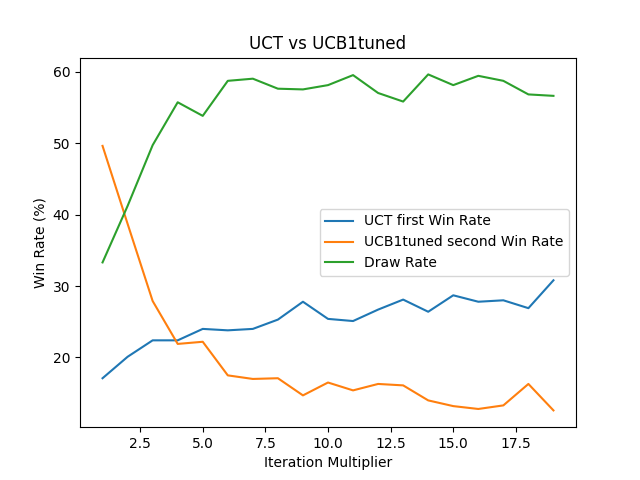
\includegraphics[width=\textwidth]{mcts/figs/40/UCT vs UCB1tuned2.png}
        \caption{UCT vs UCB1-tuned with itermax 40}
        \label{fig:401}
    \end{minipage}
    \hfill
    \begin{minipage}{0.32\textwidth}
        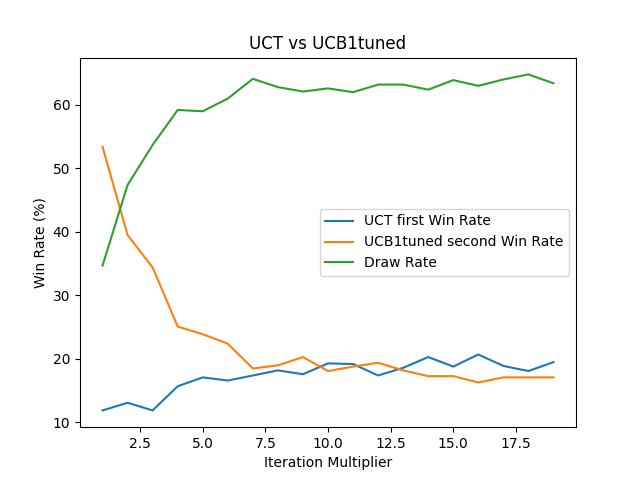
\includegraphics[width=\textwidth]{mcts/figs/80/UCT vs UCB1tuned2.png}
        \caption{UCT values UCB1-tuned with itermax 80}
        \label{fig:801}
    \end{minipage}
    \hfill
    \begin{minipage}{0.32\textwidth}
        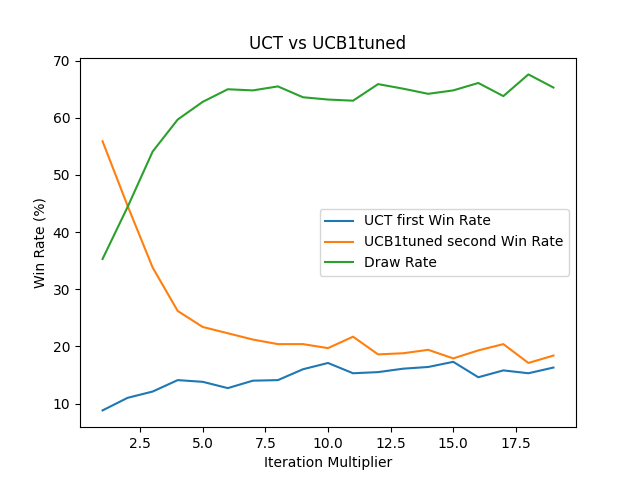
\includegraphics[width=\textwidth]{mcts/figs/120/UCT vs UCB1tuned2.png}
        \caption{UCT vs UCB1-tuned with itermax 120}
        \label{fig:1201}
    \end{minipage}
\end{figure}
\begin{figure}[H]
    \centering
    \begin{minipage}{0.32\textwidth}
        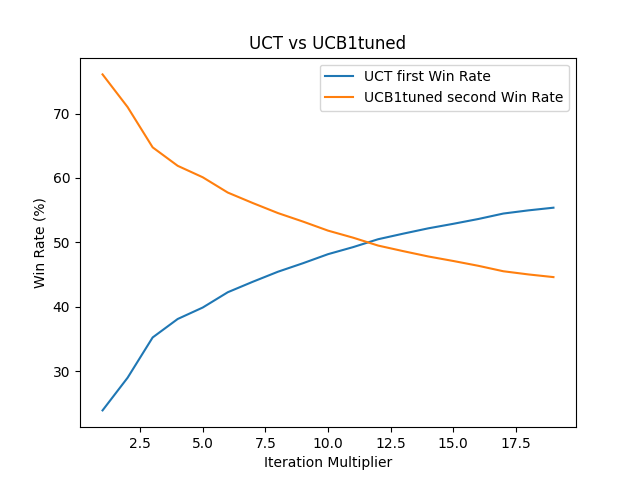
\includegraphics[width=\textwidth]{mcts/figs/40/UCT vs UCB1tuned1.png}
        \caption{UCB1-tuned vs UCT with itermax 40}
        \label{fig:402}
    \end{minipage}
    \hfill
    \begin{minipage}{0.32\textwidth}
        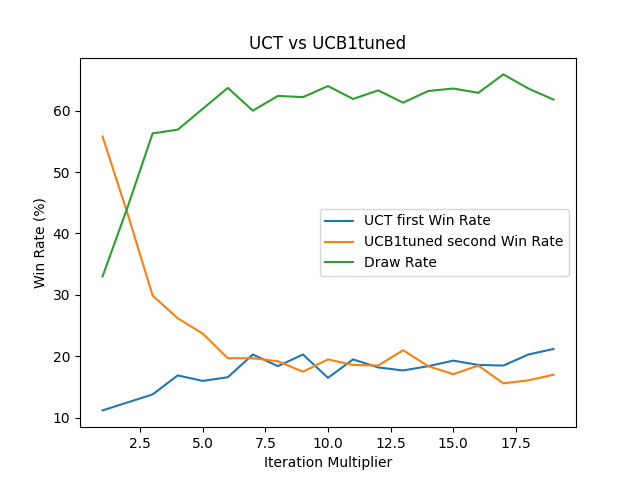
\includegraphics[width=\textwidth]{mcts/figs/80/UCT vs UCB1tuned1.png}
        \caption{UCB1-tuned vs UCT with itermax 80}
        \label{fig:802}
    \end{minipage}
    \hfill
    \begin{minipage}{0.32\textwidth}
        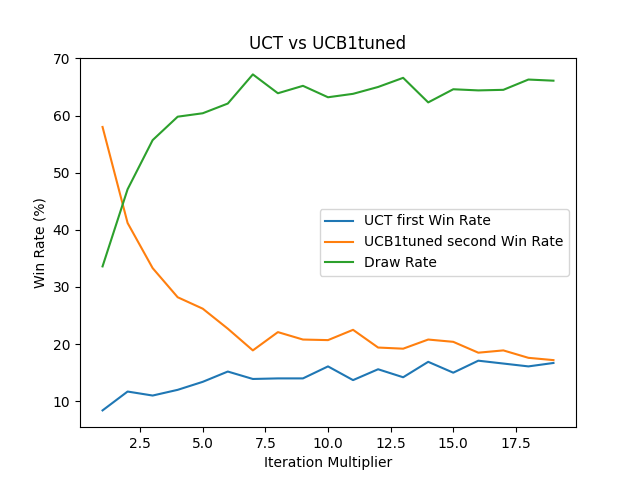
\includegraphics[width=\textwidth]{mcts/figs/120/UCT vs UCB1tuned1.png}
        \caption{UCB1-tuned vs UCT with itermax 120}
        \label{fig:1202}
    \end{minipage}
\end{figure}
For more result, you can look at the repository, the \texttt{mcts/figs} directory contains all test result and we can not list all of them due to the limitation of space.
\subsection{Conclusion}
From both the table and graph, we can see that UCT and UCB1-tuned have a state-of-the-art result, outperform other kinds of search algorithm. As the FPU mentioned, UCB1-tuned is indeed a better algorithm in application that can handle unexplored nodes and save memory better.\\
Also, since tictactoe is a relative simple game and easy to get a draw if the agents have a strong prediction power, we can see that the draw rate is higher with a deeper search.
\section{Gobang}
\subsection{Introduction}
In this task, we mainly combine the algorithm of UCTtuned(the algorithm that I finetuned) and UCT in the game of Gobang.\\
Since the board of Gobang is larger than tictactoe, we can evaluate different kind of search algorithm's ability better.
\subsection{New Algorithm}
To balance the exploration weight for different nodes better, we combine the UCT and SP-MCTS algorithm. I notice that the main part tuned in SP-MCTS is the variance tail. Since we are playing a two-player game, we do not need a hyperparameter $D$ at the summation part. Instead of that, we multiple the variance tail with a hyperparameter $D$.
\[
    \arg\max_{v'\in\text{children(v)}}\left(\frac{Q(v')}{N(v')}+C\cdot\sqrt{\frac{\log N(v)}{N(v')}}+D\cdot var(\frac{N(u)\text{ where u is v's descendent}}{N(v)})\right)
\]
\subsection{Main Code}
\begin{itemize}
    \item \texttt{Board.py}: definition of the board, provide function for user move and board update etc.
    \item \texttt{Node.py}: Basic MCTS node, used for tree updating
    \item \texttt{MCTS.py}: MCTS Algorithms, used for decide node expansion and back-propogation algorithm
    \item \texttt{Players.py}: Player Agents, used for playground GUI or AI vs AI evaluation 
\end{itemize}
\section{Conclusion}
In this survey, we have delved into the intricacies of Monte Carlo Tree Search (MCTS), exploring its foundational concepts, various algorithmic implementations, and practical applications. We began by discussing the background of MCTS, including the essential elements of Markov Decision Processes (MDP) and Monte Carlo methods. This provided a solid foundation for understanding how MCTS operates and its relevance in decision-making processes.\\
We then introduced the general MCTS algorithm, breaking down its four main steps: selection, expansion, simulation, and backpropagation. This was followed by a detailed examination of specific MCTS variants, such as reward-based MCTS, visited-based MCTS, and hybrid MCTS, highlighting their unique approaches to balancing exploration and exploitation.\\
The survey also covered state-of-the-art algorithms like UCT (Upper Confidence bounds for Trees) and its variations, including UCB1-tuned and Bayesian UCT. These algorithms were analyzed in terms of their theoretical underpinnings, practical implementations, and performance improvements over basic MCTS.\\
Furthermore, we explored the integration of learning techniques within MCTS, such as Temporal Difference (TD) learning and its Monte Carlo variant (TDMC). These methods enhance the MCTS framework by incorporating value function approximations and reducing variance in value estimation.\\
Our experimental results, particularly in the context of the Tic-Tac-Toe game, demonstrated the effectiveness of advanced MCTS algorithms like UCT and UCB1-tuned. These algorithms consistently outperformed simpler variants, showcasing their robustness and adaptability in various scenarios.\\
In conclusion, MCTS remains a powerful and versatile tool in the realm of artificial intelligence and decision-making. Its ability to balance exploration and exploitation, coupled with advancements in algorithmic strategies, ensures its continued relevance and applicability in solving complex problems. Future research and development in this field will likely yield even more sophisticated and efficient algorithms, further expanding the horizons of what MCTS can achieve.
\bibliography{reference}
\bibliographystyle{plain}
\end{document}
